\documentclass[11pt,a4paper]{article}
\usepackage[margin=1.8cm]{geometry}
\usepackage{amsmath,amssymb}
\usepackage{booktabs,array,tabularx}
\usepackage{tcolorbox}
\usepackage{microtype}
\usepackage{parskip}
\usepackage{enumitem}
\usepackage{xcolor}
\usepackage{tikz}
\usetikzlibrary{arrows.meta,positioning}
\tcbuselibrary{skins,breakable}

% ── B&W only box styles ───────────────────────────────────────────────────────
\tcbset{
  defn/.style={colback=gray!8,colframe=black,fonttitle=\bfseries\small,
    title=#1,left=4pt,right=4pt,top=3pt,bottom=3pt,boxrule=0.7pt,arc=2pt},
  bold/.style={colback=white,colframe=black,fonttitle=\bfseries\small,
    title=#1,left=4pt,right=4pt,top=3pt,bottom=3pt,boxrule=1.2pt,arc=2pt},
  exam/.style={colback=gray!5,colframe=black,fonttitle=\bfseries\small,
    title=#1,left=4pt,right=4pt,top=3pt,bottom=3pt,
    boxrule=0.5pt,arc=2pt,borderline west={2pt}{0pt}{black}},
  note/.style={colback=white,colframe=gray!60,fonttitle=\bfseries\small,
    title=#1,left=4pt,right=4pt,top=3pt,bottom=3pt,boxrule=0.5pt,arc=2pt}
}
\setlist[itemize]{noitemsep,topsep=3pt,parsep=0pt}
\setlist[enumerate]{noitemsep,topsep=3pt,parsep=0pt}

\begin{document}

% ── Title ────────────────────────────────────────────────────────────────────
\begin{center}
  {\large\bfseries DRL Sessions 4 \& 5 — MDP Formulation \& Dynamic Programming (Exam Handout)}\\[2pt]
  {\small Session 4: MDP, 3 signals, returns, discounting, G\(_t\) recursion \quad|\quad
   Session 5: Policy Evaluation, Improvement, Iteration, Value Iteration, GPI, Async DP}
\end{center}
\hrule\vspace{6pt}

% ════════════════════════════════════════════════════════════════════════════
\section*{Session 4 — MDP Formulation}
% ════════════════════════════════════════════════════════════════════════════

% ── §1 MDP Definition ───────────────────────────────────────────────────────
\subsection*{1 · What is an MDP?}

\begin{tcolorbox}[defn={Markov Decision Process (MDP)}]
An MDP is a mathematically precise formulation of the RL problem.
It consists of:
\[
  \langle \mathcal{S},\; \mathcal{A},\; \mathcal{R},\; p,\; \gamma \rangle
\]
\begin{itemize}
  \item $\mathcal{S}$ — finite set of \textbf{states}
  \item $\mathcal{A}$ — finite set of \textbf{actions}
  \item $\mathcal{R}$ — set of \textbf{rewards} (real-valued scalars)
  \item $p(s', r \mid s, a)$ — \textbf{dynamics function} (transition + reward probabilities)
  \item $\gamma$ — \textbf{discount factor}, $0 \leq \gamma \leq 1$
\end{itemize}
\end{tcolorbox}

\textbf{The Markov Property:} The future depends \emph{only} on the current state, not on the history.
\[
  P(S_{t+1}, R_{t+1} \mid S_t, A_t) = P(S_{t+1}, R_{t+1} \mid S_0, A_0, \ldots, S_t, A_t)
\]

% ── §2 Three signals ────────────────────────────────────────────────────────
\subsection*{2 · The 3 Signals Between Agent and Environment}

\begin{tcolorbox}[bold={Three Signals — Must Know}]
\begin{center}
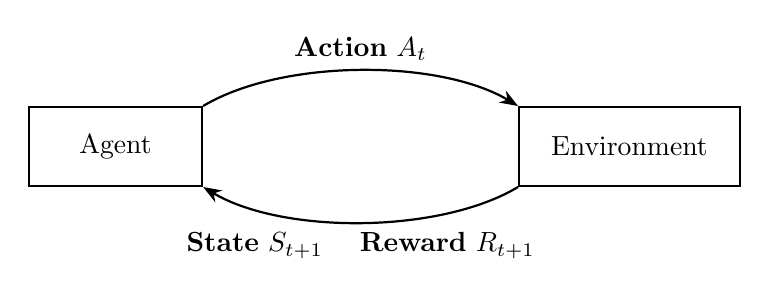
\begin{tikzpicture}[node distance=1.2cm,>=Stealth]
  \node[draw,thick,minimum width=2.2cm,minimum height=1cm] (agent) {Agent};
  \node[draw,thick,minimum width=2.8cm,minimum height=1cm,right=4cm of agent] (env) {Environment};
  % top arrow: Action
  \draw[->,thick] (agent.north east) .. controls +(1,0.6) and +(-1,0.6) .. (env.north west)
    node[midway,above]{\textbf{Action} $A_t$};
  % bottom arrows: State and Reward
  \draw[->,thick] (env.south west) .. controls +(-1,-0.6) and +(1,-0.6) .. (agent.south east)
    node[midway,below]{\textbf{State} $S_{t+1}$ \quad \textbf{Reward} $R_{t+1}$};
\end{tikzpicture}
\end{center}
\vspace{4pt}
\begin{tabular}{p{2.4cm}p{3.6cm}p{8cm}}
\textbf{Signal} & \textbf{Direction} & \textbf{Meaning} \\
\midrule
$S_t$ (State) & Environment $\to$ Agent & Current situation the agent observes \\
$A_t$ (Action) & Agent $\to$ Environment & Decision taken at step $t$ \\
$R_{t+1}$ (Reward) & Environment $\to$ Agent & Scalar feedback after taking $A_t$ in $S_t$ \\
\end{tabular}

\medskip
\textbf{Dynamics function:}
$\displaystyle p(s', r \mid s, a) = \Pr\{S_{t+1}=s',\, R_{t+1}=r \mid S_t=s,\, A_t=a\}$
\end{tcolorbox}

% ── §3 Returns and Discounting ───────────────────────────────────────────────
\subsection*{3 · Returns, Discounting, and $G_t$}

\textbf{Goal:} Maximise the \textbf{expected return} $G_t$ — not just the next reward, but the
cumulative future reward.

\begin{tcolorbox}[defn={Discounted Return}]
\[
  G_t \;=\; R_{t+1} + \gamma R_{t+2} + \gamma^2 R_{t+3} + \cdots
       \;=\; \sum_{k=0}^{\infty} \gamma^k R_{t+k+1}
\]
\end{tcolorbox}

\textbf{Role of $\gamma$ (discount factor):}
\begin{center}
\begin{tabular}{p{2.5cm}p{5.5cm}p{5.5cm}}
\toprule
$\gamma$ & Effect & Use case \\
\midrule
$\gamma = 0$ & Only immediate reward matters (myopic) & Short-horizon tasks; immediate payoff \\
$0 < \gamma < 1$ & Future rewards discounted exponentially & Most practical RL tasks \\
$\gamma = 1$ & All future rewards count equally & Episodic tasks with finite horizon only \\
\bottomrule
\end{tabular}
\end{center}

\textbf{Why discount?}
\begin{enumerate}
  \item Mathematical convergence: guarantees $G_t$ is finite when rewards are bounded.
  \item Economic interpretation: a reward now is worth more than the same reward later (time preference).
  \item Uncertainty: future transitions may not occur as expected; discounting hedges against this.
\end{enumerate}

% ── §4 Episodic vs Continuing ────────────────────────────────────────────────
\subsection*{4 · Episodic vs.\ Continuing Tasks}

\begin{tcolorbox}[defn={Two Task Types}]
\begin{tabular}{p{3.5cm}p{5.5cm}p{5cm}}
\toprule
& \textbf{Episodic} & \textbf{Continuing} \\
\midrule
Termination & Has a terminal state $T$ & Runs forever \\
Return formula & $G_t = \displaystyle\sum_{k=0}^{T-t-1} R_{t+k+1}$ (no $\gamma$ needed) & $G_t = \displaystyle\sum_{k=0}^{\infty} \gamma^k R_{t+k+1}$ (need $\gamma<1$) \\
Examples & Chess, Tic-Tac-Toe, maze & Trading bot, robot control \\
$\gamma = 1$ allowed? & Yes (finite sum) & No (infinite sum diverges) \\
\bottomrule
\end{tabular}
\end{tcolorbox}

\textbf{Unified formula} (using absorbing terminal state with zero reward):
\[
  G_t = \sum_{k=t+1}^{T} \gamma^{k-t-1} R_k \quad \text{(works for both; set } T=\infty \text{ for continuing)}
\]

% ── §5 Recursive formulation ─────────────────────────────────────────────────
\subsection*{5 · Recursive Formulation — $G_t$ in terms of $G_{t+1}$}

\begin{tcolorbox}[bold={Key Recursion — used in every RL algorithm}]
\[
  G_t \;=\; R_{t+1} + \gamma G_{t+1}
\]
\end{tcolorbox}

\textbf{Derivation (one step):}
\begin{align*}
  G_t &= R_{t+1} + \gamma R_{t+2} + \gamma^2 R_{t+3} + \cdots \\
      &= R_{t+1} + \gamma \bigl( R_{t+2} + \gamma R_{t+3} + \cdots \bigr) \\
      &= R_{t+1} + \gamma G_{t+1}
\end{align*}

\textbf{Why is this useful?}
\begin{itemize}
  \item Allows computing $G_t$ \emph{backwards} from the terminal state — no need to store the full trajectory.
  \item Directly motivates the TD update: estimate $G_t \approx R_{t+1} + \gamma V(S_{t+1})$.
  \item The Bellman equations (next section) are built entirely on this recursion.
\end{itemize}

% ── §6 Value Functions ───────────────────────────────────────────────────────
\subsection*{6 · Value Functions and Bellman Equation}

\begin{tcolorbox}[defn={State-value and action-value functions}]
\[
  v_\pi(s) \;=\; \mathbb{E}_\pi[G_t \mid S_t = s]
           \;=\; \sum_a \pi(a|s) \sum_{s',r} p(s',r|s,a)\bigl[r + \gamma v_\pi(s')\bigr]
\]
\[
  q_\pi(s,a) \;=\; \mathbb{E}_\pi[G_t \mid S_t = s,\, A_t = a]
             \;=\; \sum_{s',r} p(s',r|s,a)\bigl[r + \gamma v_\pi(s')\bigr]
\]
The first equation is the \textbf{Bellman equation} for $v_\pi$.
\end{tcolorbox}

\hrule\vspace{8pt}

% ════════════════════════════════════════════════════════════════════════════
\section*{Session 5 — Dynamic Programming (DP)}
% ════════════════════════════════════════════════════════════════════════════

\subsection*{7 · Characteristics of DP}

\begin{tcolorbox}[defn={What is DP in the RL context?}]
DP refers to a collection of algorithms that use the \textbf{Bellman equations} to compute
optimal value functions, given a \textbf{perfect model} of the environment.
\end{tcolorbox}

\textbf{Characteristics:}
\begin{enumerate}
  \item Requires a \textbf{complete model}: $p(s', r \mid s, a)$ must be fully known.
  \item Computationally \textbf{expensive} for large state spaces, but \textbf{exact}.
  \item Uses \textbf{bootstrapping}: updates are based on estimates of other states (not sampled rewards alone).
  \item Finds the \textbf{optimal policy} $\pi^*$ and optimal value function $v^*$.
\end{enumerate}

\textbf{When DP is applicable:}
\begin{itemize}
  \item State and action spaces are \textbf{finite} and \textbf{small}.
  \item The full transition model $p(s',r|s,a)$ is \textbf{known} (not needed to interact with real world).
  \item Examples: grid worlds, small board games, Jack's Car Rental, Gambler's Problem.
  \item Not applicable: large/continuous spaces (use function approximation), unknown model (use MC or TD).
\end{itemize}

% ── §8 Key Terms ─────────────────────────────────────────────────────────────
\subsection*{8 · Key Terms (Policy Evaluation → Value Iteration)}

\begin{tcolorbox}[exam={Five Key Terms — Know Each Precisely}]
\textbf{(1) Policy Evaluation} (Prediction Problem)\\
\quad Given policy $\pi$, compute $v_\pi(s)$ for all states. Use iterative sweeps:
\[
  v_{k+1}(s) = \sum_a \pi(a|s) \sum_{s',r} p(s',r|s,a)\bigl[r + \gamma v_k(s')\bigr]
\]
Repeat until $\max_s |v_{k+1}(s) - v_k(s)| < \theta$ (some small threshold).

\medskip
\textbf{(2) Policy Improvement} (Control — one step)\\
\quad Given $v_\pi$, form a \emph{greedy} policy $\pi'$:
\[
  \pi'(s) = \arg\max_a \sum_{s',r} p(s',r|s,a)\bigl[r + \gamma v_\pi(s')\bigr]
\]
\textbf{Policy Improvement Theorem:} $v_{\pi'}(s) \geq v_\pi(s)$ for all $s$
(the new greedy policy is at least as good as the old one).

\medskip
\textbf{(3) Policy Iteration}\\
\quad Alternate: full Policy Evaluation $\to$ full Policy Improvement $\to$ repeat.\\
Converges to $\pi^*$ in a finite number of iterations (finite MDP).

\medskip
\textbf{(4) Value Iteration}\\
\quad Combine one sweep of (partial) evaluation + improvement:
\[
  v_{k+1}(s) = \max_a \sum_{s',r} p(s',r|s,a)\bigl[r + \gamma v_k(s')\bigr]
\]
No need to wait for full policy evaluation to converge between improvements.
Faster in practice.

\medskip
\textbf{(5) Generalized Policy Iteration (GPI)}\\
\quad The general idea of \emph{any} interleaving of evaluation and improvement, regardless of granularity.
All RL algorithms are a form of GPI.
\end{tcolorbox}

\begin{tcolorbox}[note={Asynchronous DP}]
Standard DP sweeps all states uniformly (synchronous). \textbf{Asynchronous DP} updates states
in any order — it can focus on states that are most relevant (e.g., those the agent visits often).
\begin{itemize}
  \item Useful for large state spaces.
  \item Still requires a full model.
  \item Converges as long as every state is updated infinitely often in the limit.
\end{itemize}
\end{tcolorbox}

% ── §9 Comparison: Policy Iter vs Value Iter ─────────────────────────────────
\subsection*{9 · Policy Iteration vs.\ Value Iteration}

\begin{center}
\begin{tabular}{p{4cm}p{5.5cm}p{5.5cm}}
\toprule
& \textbf{Policy Iteration} & \textbf{Value Iteration} \\
\midrule
Evaluation step & Run full Bellman expectation until convergence & One Bellman \emph{optimality} sweep \\
Improvement step & Full greedy improvement after evaluation & Combined into same sweep \\
Iterations & Fewer policy updates, each costly & More iterations but each cheap \\
Update per step & $v_{k+1}(s) = \sum_a \pi(a|s)[\ldots]$ & $v_{k+1}(s) = \max_a [\ldots]$ \\
Convergence & Finite (finite MDP) & Geometric ($\gamma^k$ contraction) \\
When to prefer & When evaluation is cheap; small MDP & When model is known but large \\
\bottomrule
\end{tabular}
\end{center}

% ── §10 Worked Example ───────────────────────────────────────────────────────
\subsection*{10 · Worked Example — Value Iteration (Race Car / 1-D Track)}

\begin{tcolorbox}[exam={Race Car Problem (Simplified)}]
\textbf{Setup:} A car is on a 1-D track: states $s \in \{0, 1, 2, 3, 4\}$ (positions).
State 4 = \textbf{Finish} (terminal). Actions: \texttt{Fast} (move 2 positions forward, reward $-1$)
or \texttt{Slow} (move 1 position forward, reward $-1$). Goal: reach state 4 in minimum steps.
Discount $\gamma = 0.9$. All transitions are deterministic.

\medskip
\textbf{Initialise:} $v_0(s) = 0$ for all $s$. $v(4) = 0$ always (terminal).

\medskip
\textbf{Iteration 1 — Value Iteration sweep} (apply $v_{k+1}(s) = \max_a[r + \gamma v_k(s')]$):

\smallskip
From state 3: Fast $\to$ 5 (out of range/clamped to 4), Slow $\to$ 4.
Both reach finish: $r = -1$, $v_0(4) = 0$.
\[ v_1(3) = \max(-1 + 0.9\times0,\ -1 + 0.9\times0) = -1 \]

From state 2: Fast $\to$ 4 ($r=-1$, $v_0(4)=0$); Slow $\to$ 3 ($r=-1$, $v_0(3)=0$).
\[ v_1(2) = \max(-1 + 0,\ -1 + 0) = -1 \]

From state 1: Fast $\to$ 3 ($r=-1$, $v_0(3)=0$); Slow $\to$ 2 ($r=-1$, $v_0(2)=0$).
\[ v_1(1) = -1 \]

From state 0: Fast $\to$ 2; Slow $\to$ 1. Both: $-1$.
\[ v_1(0) = -1 \]

\medskip
\textbf{Iteration 2:}

From state 3: same as before $= -1$.

From state 2: Fast $\to$ 4 ($-1 + 0 = -1$); Slow $\to$ 3 ($-1 + 0.9\times(-1) = -1.9$).
\[ v_2(2) = \max(-1,\ -1.9) = -1 \quad \Rightarrow \text{prefer \texttt{Fast}} \]

From state 1: Fast $\to$ 3 ($-1 + 0.9\times(-1) = -1.9$); Slow $\to$ 2 ($-1 + 0.9\times(-1) = -1.9$).
\[ v_2(1) = -1.9 \]

From state 0: Fast $\to$ 2 ($-1 + 0.9\times(-1) = -1.9$); Slow $\to$ 1 ($-1 + 0.9\times(-1.9)=-2.71$).
\[ v_2(0) = \max(-1.9,\ -2.71) = -1.9 \quad \Rightarrow \text{prefer \texttt{Fast}} \]

\textbf{Emerging policy:} always take \texttt{Fast} — reach finish in fewest steps.
Values converge downward as they properly account for the number of steps to terminal.
\end{tcolorbox}

% ── §11 GPI Diagram ──────────────────────────────────────────────────────────
\subsection*{11 · Generalized Policy Iteration (GPI) — The Big Picture}

\begin{tcolorbox}[defn={GPI — All RL is GPI}]
\[
  \pi \;\xrightarrow{\text{Evaluate}}\; v_\pi \;\xrightarrow{\text{Improve}}\; \pi' \;\xrightarrow{\text{Evaluate}}\; v_{\pi'} \;\xrightarrow{\text{Improve}}\; \cdots \;\to\; \pi^*, v^*
\]
\begin{itemize}
  \item \textbf{Evaluation} drives $v$ toward $v_\pi$ (makes value consistent with current policy).
  \item \textbf{Improvement} drives $\pi$ toward greedy w.r.t.\ current $v$ (makes policy consistent with value).
  \item These two goals are \emph{competing} (each step invalidates the other) but converge to a stable solution where $\pi = \text{greedy}(v_\pi) = \pi^*$.
  \item Every RL method — MC, TD, actor-critic — is a specific instance of GPI.
\end{itemize}
\end{tcolorbox}

% ── §12 Exam Points ──────────────────────────────────────────────────────────
\subsection*{12 · Exam Key-Takeaways}

\begin{tcolorbox}[exam={Must Know — Sessions 4 \& 5}]
\begin{enumerate}
  \item \textbf{3 signals:} state $S_t$ (env$\to$agent), action $A_t$ (agent$\to$env), reward $R_{t+1}$ (env$\to$agent).
  \item \textbf{Discount $\gamma$:} $\gamma=0$ myopic; $\gamma=1$ only for episodic; $0<\gamma<1$ in practice.
  \item \textbf{Episodic vs continuing:} episodic has terminal state $T$; continuing needs $\gamma<1$ for convergence.
  \item \textbf{$G_t$ recursion:} $G_t = R_{t+1} + \gamma G_{t+1}$ — memorise and be able to derive.
  \item \textbf{Bellman equation:} $v_\pi(s) = \sum_a \pi(a|s)\sum_{s',r} p(s',r|s,a)[r + \gamma v_\pi(s')]$.
  \item \textbf{Policy Eval:} use Bellman expectation iteratively for given $\pi$.
  \item \textbf{Value Iter:} use Bellman \emph{optimality} — $\max_a$ replaces $\sum_a\pi(a|s)$.
  \item \textbf{Policy Iter vs Value Iter:} Policy Iter waits for full eval; Value Iter doesn't.
  \item \textbf{GPI:} any interleaving of evaluation + improvement converges to $\pi^*$.
  \item \textbf{Async DP:} update states in any order; still needs full model; useful for large $|\mathcal{S}|$.
\end{enumerate}
\end{tcolorbox}

\vspace{4pt}
\hrule
\vspace{3pt}
{\footnotesize DRL EC3 Exam Handout — Sessions 4 \& 5 (MDP \& Dynamic Programming). Ref: Sutton \& Barto Ch.~3--4.}

\end{document}
